\documentclass[11pt,a4paper]{article}
\usepackage[margin=2.5cm]{geometry}
\usepackage{graphicx}
\usepackage{amsmath,amssymb}
\usepackage{booktabs}
\usepackage{hyperref}
\usepackage{float}
\usepackage[T1]{fontenc}
\usepackage{mathptmx}
\usepackage{microtype}
\usepackage{enumitem}
\usepackage[dvipsnames]{xcolor}
\usepackage{tcolorbox}
\tcbuselibrary{skins,breakable}

\hypersetup{colorlinks=true,linkcolor=RoyalBlue,citecolor=RoyalBlue,urlcolor=RoyalBlue}

\newtcolorbox{keyidea}[1][]{
  colback=blue!5!white, colframe=RoyalBlue!75!black,
  fonttitle=\bfseries, title={Key Idea}, #1
}
\newtcolorbox{warning}[1][]{
  colback=red!5!white, colframe=BrickRed!75!black,
  fonttitle=\bfseries, title={Why This Matters}, #1
}
\newtcolorbox{config}[1][]{
  colback=green!5!white, colframe=ForestGreen!75!black,
  fonttitle=\bfseries, title={Your Configuration}, #1
}

\title{\LARGE\bfseries Datum Projection, 2D Mode, and Map Frame\\[6pt]
\large A Deep Dive into How Your EKF Decides\\
``Where Am I on Earth?'' and ``What Is My Map Origin?''}
\author{Reference Guide for the Multi-Sensor Fusion Project}
\date{May 2026}

\begin{document}
\maketitle
\tableofcontents
\newpage

% ============================================================
\section{The Big Picture: What Problem Are We Solving?}
% ============================================================

Your robot lives in a Gazebo simulation. It has a GPS sensor that reports
latitude and longitude (e.g., $49.9^\circ$N, $8.9^\circ$E). But your EKF
works in \emph{meters}---it tracks position as $(x, y)$ on a flat 2D plane.

So the fundamental questions are:
\begin{enumerate}
  \item \textbf{How do we go from lat/lon (curved Earth) to meters (flat plane)?}
        $\rightarrow$ This is the \emph{datum projection} problem.
  \item \textbf{Where is $(0, 0)$ on that flat plane?}
        $\rightarrow$ This is the \emph{datum origin} (map origin) problem.
  \item \textbf{Which direction is ``forward'' ($+X$)?}
        $\rightarrow$ This is the \emph{heading alignment} problem.
  \item \textbf{Why do we only track $x, y, \psi$ and not $z$, roll, pitch?}
        $\rightarrow$ This is the \emph{2D mode} choice.
\end{enumerate}

This document walks through each of these, showing exactly how your project's
configuration files answer each question.

% ============================================================
\section{Step 1: The Gazebo World Defines ``Where on Earth''}
% ============================================================

\subsection{Spherical Coordinates in \texttt{agriculture.world}}

The Gazebo world file contains this block:

\begin{verbatim}
  <spherical_coordinates>
    <surface_model>EARTH_WGS84</surface_model>
    <world_frame_orientation>ENU</world_frame_orientation>
    <latitude_deg>49.9</latitude_deg>
    <longitude_deg>8.9</longitude_deg>
    <elevation>0</elevation>
    <heading_deg>0</heading_deg>
  </spherical_coordinates>
\end{verbatim}

What each line means:

\begin{description}[leftmargin=2em]
  \item[\texttt{EARTH\_WGS84}] --- The Earth is modeled as the WGS-84
    ellipsoid, the same mathematical shape that every GPS satellite uses.
    It's not a perfect sphere---it's slightly squished at the poles
    (equatorial radius = 6378.137\,km, polar radius = 6356.752\,km).

  \item[\texttt{ENU}] --- ``East--North--Up.'' This tells Gazebo how to
    orient its $X, Y, Z$ axes relative to the Earth:
    \begin{itemize}
      \item $+X$ = East
      \item $+Y$ = North
      \item $+Z$ = Up
    \end{itemize}

  \item[\texttt{latitude=49.9, longitude=8.9}] --- The Gazebo world origin
    $(0, 0, 0)$ corresponds to this point on Earth. It's near Darmstadt,
    Germany. When the robot is at Gazebo position $(0, 0, 0)$, the GPS sensor
    will report approximately $49.9^\circ$N, $8.9^\circ$E.

  \item[\texttt{heading=0}] --- No rotation between the ENU geographic frame
    and the Gazebo world frame. Gazebo $+X$ \emph{is} geographic East.
\end{description}

\begin{keyidea}
The spherical coordinates block is what makes GPS work in Gazebo. Without it,
the NavSat plugin has no way to convert the robot's $(x, y, z)$ position in
the simulator back to latitude/longitude. It defines the ``anchor point''
between the simulated flat world and the curved Earth.
\end{keyidea}

\subsection{How the NavSat Sensor Generates GPS Readings}

The \texttt{gz::sim::systems::NavSat} plugin does this every 0.1\,s (10\,Hz):
\begin{enumerate}
  \item Read the robot's current Gazebo pose: $(x_{\text{gz}}, y_{\text{gz}}, z_{\text{gz}})$ in meters.
  \item Use the WGS-84 inverse projection to convert this to $(\varphi, \lambda, h)$:
    \begin{align}
      \varphi &= \varphi_0 + \frac{y_{\text{gz}}}{R_{\text{meridian}}} \cdot \frac{180}{\pi} \\
      \lambda &= \lambda_0 + \frac{x_{\text{gz}}}{R_{\text{prime}} \cos\varphi_0} \cdot \frac{180}{\pi}
    \end{align}
    where $R_{\text{meridian}} \approx 6.366 \times 10^6$\,m and $R_{\text{prime}} \approx 6.389 \times 10^6$\,m at $49.9^\circ$N.
  \item Add Gaussian noise: $\sigma_{\text{horiz}} = 4.5 \times 10^{-6}$\,deg $\approx 0.5$\,m.
  \item Publish as \texttt{sensor\_msgs/NavSatFix} on \texttt{/gps/fix}.
\end{enumerate}

\begin{warning}
The noise is specified in \emph{degrees}, not meters! At this latitude,
$1^\circ$ latitude $\approx 111$\,km. So $4.5 \times 10^{-6}$ degrees
$\approx 0.5$\,m. This is a common source of confusion when configuring
Gazebo GPS sensors.
\end{warning}

% ============================================================
\section{Step 2: From Lat/Lon to Local XY Meters}
% ============================================================

\subsection{The UTM Projection}

GPS gives you latitude and longitude, but your EKF thinks in meters. The
\texttt{navsat\_transform\_node} bridges this gap using the \textbf{UTM
(Universal Transverse Mercator)} projection.

\begin{figure}[H]
\centering
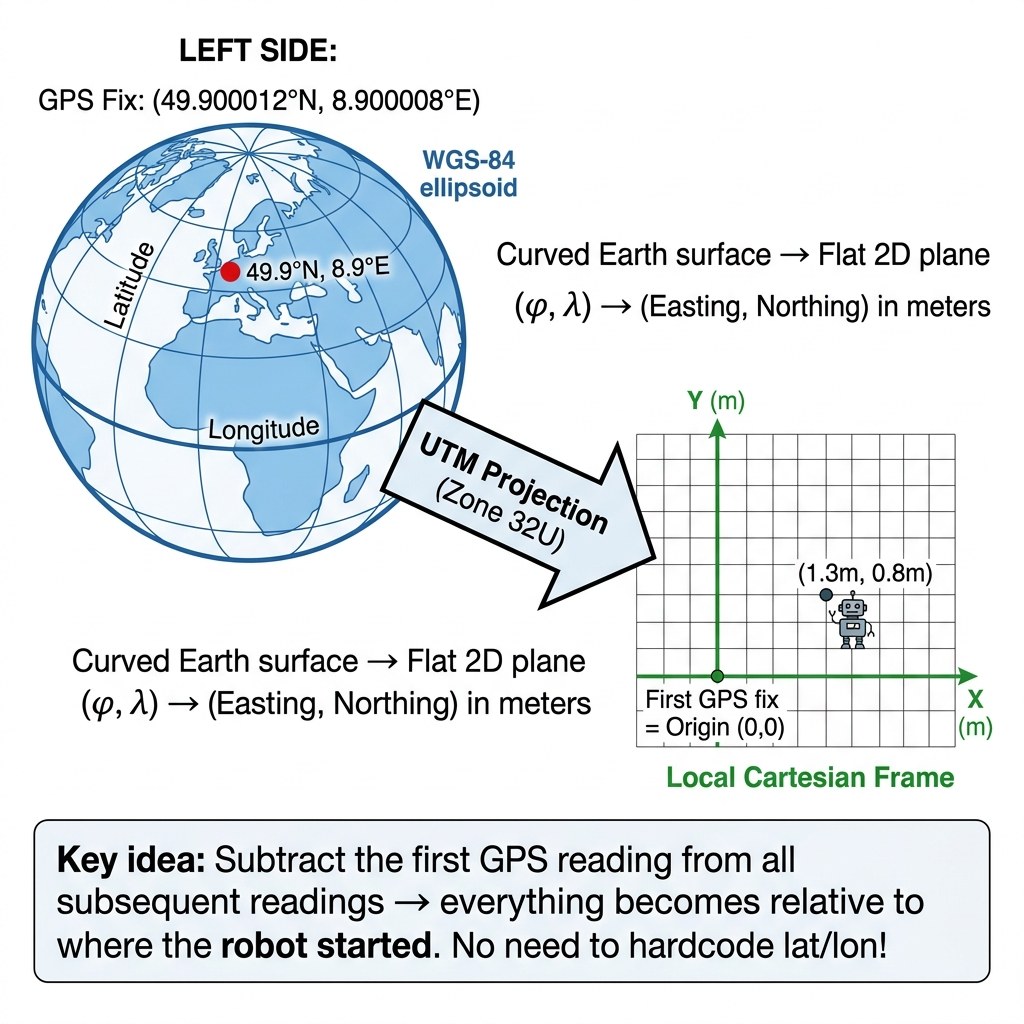
\includegraphics[width=0.85\textwidth]{figures/wgs84_utm_projection.png}
\caption{How GPS lat/lon becomes local $(x, y)$ in meters. The UTM projection
flattens the curved Earth surface, and subtracting the first GPS fix makes
everything relative to the robot's starting position.}
\label{fig:utm}
\end{figure}

UTM divides the Earth into 60 vertical strips (``zones''), each 6$^\circ$ wide.
For your world origin at $8.9^\circ$E, this falls in \textbf{Zone 32U}
(covering $6^\circ$E to $12^\circ$E). Within each zone, UTM uses a transverse
Mercator projection to convert $(\varphi, \lambda)$ to $(E, N)$ in meters:
\begin{itemize}
  \item $E$ = Easting (meters east of the zone's central meridian, offset by 500\,km)
  \item $N$ = Northing (meters north of the equator)
\end{itemize}

The key property: over your robot's $\sim$40\,m operating range, the UTM
projection introduces $< 0.04\%$ distortion. A 40\,m drive in reality
becomes 39.984\,m in UTM---a 0.016\,m error that's completely negligible
compared to your 0.5\,m GPS noise.

\subsection{The First-Fix Datum: Where Is (0, 0)?}

\begin{config}
From \texttt{baseline\_ekf.yaml}, navsat section:
\begin{verbatim}
  wait_for_datum: false
\end{verbatim}
\end{config}

\noindent This single parameter determines \emph{how the map origin is chosen}:

\begin{itemize}
  \item \texttt{wait\_for\_datum: true} would mean: ``I will tell you the exact
    lat/lon to use as $(0, 0)$.'' You'd provide a \texttt{datum} parameter
    with hardcoded coordinates.
  \item \texttt{wait\_for\_datum: false} (your setting) means: ``Use the
    \textbf{first GPS fix you receive} as the origin.''
\end{itemize}

In your system, the first GPS fix arrives at $t \approx 18$\,s (after Gazebo
loads, sensors start, and the staged launch gates pass). At that moment, the
robot is still at its spawn position $(0, 0, 0)$ in Gazebo. So:
\begin{align}
  \text{First GPS fix:} \quad &(\varphi_{\text{first}}, \lambda_{\text{first}}) \approx (49.9^\circ\text{N},\; 8.9^\circ\text{E}) \\
  \text{UTM conversion:} \quad &(E_{\text{first}}, N_{\text{first}}) = (488\,xxx\text{\,m},\; 5\,527\,xxx\text{\,m}) \\
  \text{Local origin:} \quad &(0, 0) \leftarrow \text{this position}
\end{align}

Every subsequent GPS fix is then computed as:
\begin{equation}
  (x, y)_{\text{local}} = (E - E_{\text{first}},\;\; N - N_{\text{first}})
\end{equation}

\begin{keyidea}
The map origin is wherever the robot happened to be when the navsat node
received its first GPS fix. No hardcoded coordinates needed. This is why
\texttt{wait\_for\_datum: false} is the more portable choice---your system
works in any Gazebo world without changing config files.
\end{keyidea}

% ============================================================
\section{Step 3: Heading Alignment---Which Way Is ``Forward''?}
% ============================================================

Converting lat/lon to meters gives you $(x, y)$ positions, but there's still
an ambiguity: which direction does the local $+X$ axis point? The navsat node
needs a heading reference to rotate the UTM frame into the robot's local frame.

\begin{config}
\begin{verbatim}
  use_odometry_yaw: true
  magnetic_declination_radians: 0.0
  yaw_offset: 0.0
\end{verbatim}
\end{config}

\noindent\textbf{\texttt{use\_odometry\_yaw: true}} is the critical setting. It means:

\begin{quote}
``Take the heading (yaw) from \texttt{/odometry/local} (EKF\,\#1's output),
not from the IMU's absolute orientation.''
\end{quote}

\subsection{Why Not Use IMU Yaw Directly?}

In the real world with a magnetometer, the IMU knows which way is North. But
your Gazebo IMU has \textbf{no magnetometer}. Its ``absolute'' yaw is just the
integrated gyroscope---which starts at some arbitrary value and drifts over
time ($> 150^\circ$ drift in 2 minutes!).

Worse, there's a subtler problem: even if the IMU \emph{did} report true North,
the angle between Gazebo world-$X$ and geographic East at $49.9^\circ$N is
$\sim$$58^\circ$. Using IMU yaw would rotate your entire map frame by
$58^\circ$, misaligning everything.

\subsection{How \texttt{use\_odometry\_yaw: true} Solves This}

EKF\,\#1 starts with $\psi = 0$ (the robot spawns at heading zero). At
$t = 18$\,s when navsat initializes, EKF\,\#1's heading is still
$\psi \approx 0$. The navsat node reads this and says: ``The robot's forward
direction aligns with my local $+X$ axis.'' This means:
\begin{itemize}
  \item \texttt{map} frame $+X$ = same direction as \texttt{odom} frame $+X$ at startup
  \item No mysterious rotation between frames
  \item \texttt{map}$\rightarrow$\texttt{odom} starts as identity (zero translation, zero rotation)
\end{itemize}

% ============================================================
\section{Step 4: The Three Coordinate Frames}
% ============================================================

\begin{figure}[H]
\centering
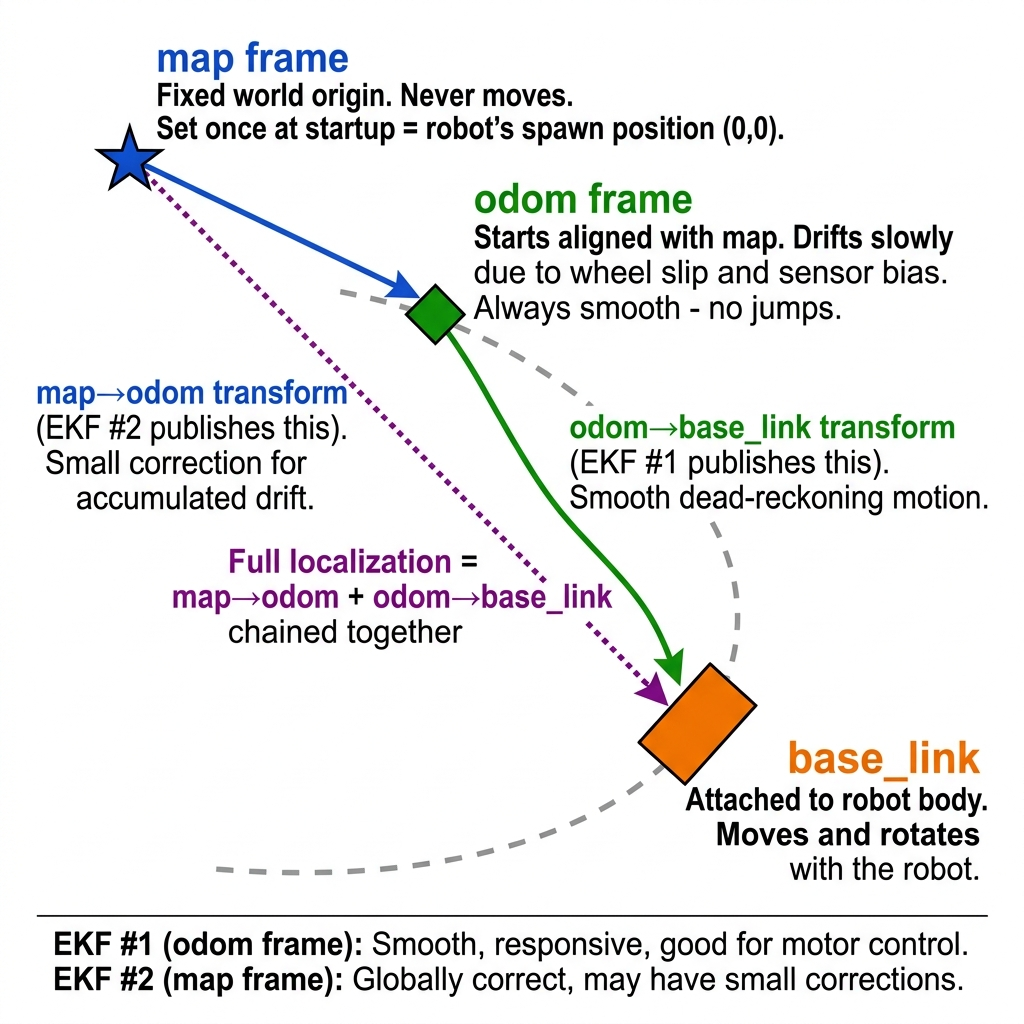
\includegraphics[width=0.85\textwidth]{figures/map_odom_baselink.png}
\caption{The three coordinate frames in the ROS\,2 TF tree. The
\texttt{map} frame is fixed, \texttt{odom} drifts smoothly, and
\texttt{base\_link} moves with the robot. Two EKFs each publish one
transform in this chain.}
\label{fig:frames}
\end{figure}

\subsection{Frame Definitions}

\begin{description}[leftmargin=2em, itemsep=6pt]
  \item[\textcolor{RoyalBlue}{\texttt{map}}] \textbf{The global fixed frame.}
    Origin = robot's spawn position. Never moves. This is where ``the world''
    is. If you ask ``where is the robot in the world?'' you want the robot's
    pose in the \texttt{map} frame.

  \item[\textcolor{ForestGreen}{\texttt{odom}}] \textbf{The smooth local
    frame.} Starts at the same place as \texttt{map}. Over time, it
    \emph{drifts} because wheel odometry accumulates small errors (wheel slip,
    uneven terrain). But it's \textbf{always smooth}---no sudden jumps. This
    makes it ideal for motion control (sending velocity commands).

  \item[\textcolor{BrickRed}{\texttt{base\_link}}] \textbf{The robot body
    frame.} Attached to the robot's center. Moves and rotates with the robot.
    All sensor data is ultimately referenced to this frame.
\end{description}

\subsection{Who Publishes What}

\begin{table}[H]
\centering
\begin{tabular}{@{}llll@{}}
\toprule
\textbf{Transform} & \textbf{Published by} & \textbf{\texttt{world\_frame}} & \textbf{Meaning} \\
\midrule
\texttt{odom}$\rightarrow$\texttt{base\_link} & EKF\,\#1 & \texttt{odom} & Smooth local motion \\
\texttt{map}$\rightarrow$\texttt{odom} & EKF\,\#2 & \texttt{map} & Drift correction \\
\bottomrule
\end{tabular}
\caption{Transform responsibilities in the dual-EKF architecture.}
\end{table}

The full robot pose in the world is the \emph{chain}:
\begin{equation}
  T_{\texttt{map}}^{\texttt{base\_link}} = T_{\texttt{map}}^{\texttt{odom}} \cdot T_{\texttt{odom}}^{\texttt{base\_link}}
\end{equation}

\begin{keyidea}
The \texttt{world\_frame} parameter in each EKF's YAML determines which
transform that EKF publishes:
\begin{itemize}
  \item \texttt{world\_frame: odom} $\Rightarrow$ publishes \texttt{odom}$\rightarrow$\texttt{base\_link}
  \item \texttt{world\_frame: map} $\Rightarrow$ publishes \texttt{map}$\rightarrow$\texttt{odom}
\end{itemize}
That's it. That single parameter controls which frame the EKF ``owns.''
\end{keyidea}

% ============================================================
\section{Step 5: 2D Mode---Projecting to the Ground Plane}
% ============================================================

\begin{figure}[H]
\centering
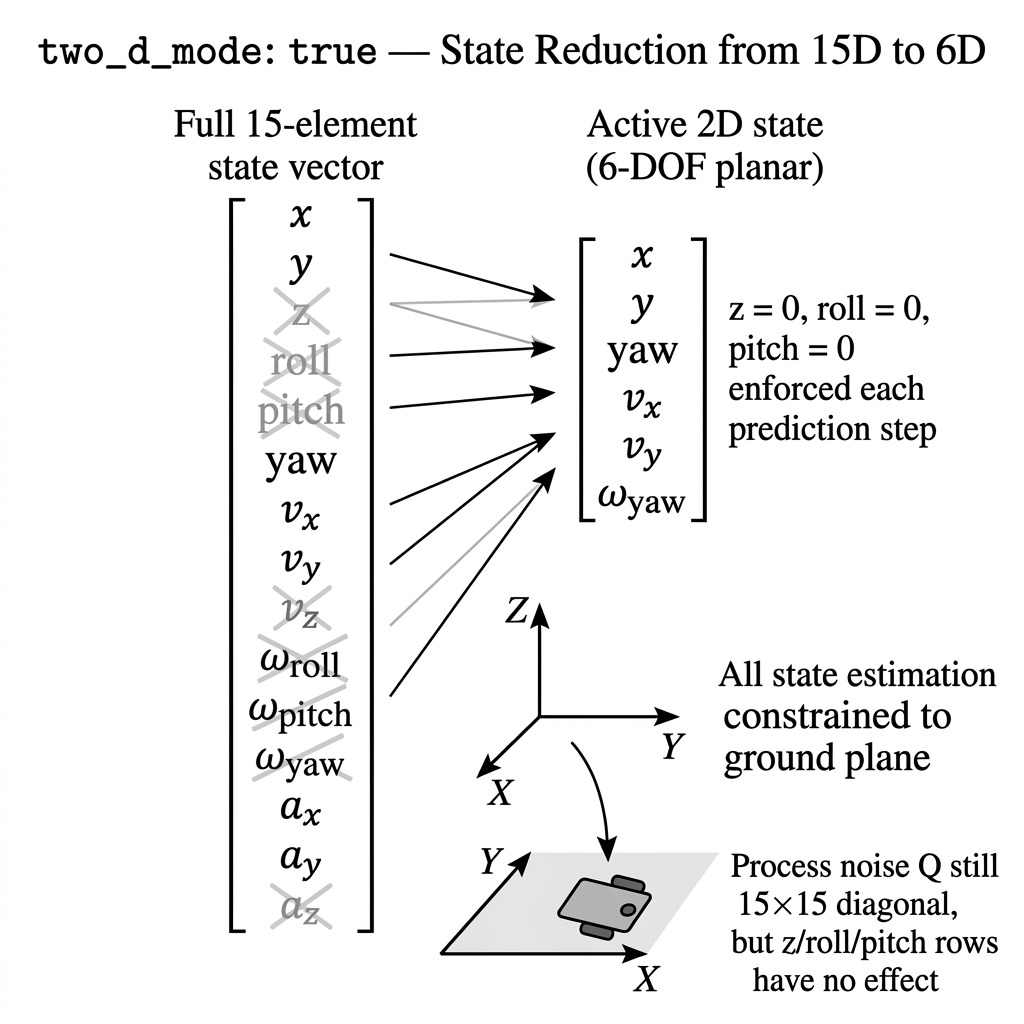
\includegraphics[width=0.8\textwidth]{figures/two_d_mode_projection.png}
\caption{The \texttt{two\_d\_mode: true} setting reduces the 15-element state
vector to an effective 6-DOF planar state. Greyed/crossed elements are zeroed
at each prediction step.}
\label{fig:2dmode}
\end{figure}

\subsection{The Full 15-Element State}

The \texttt{robot\_localization} EKF internally maintains a 15-element state:
\begin{equation}
  \mathbf{x} = \underbrace{[x, y, z}_{\text{position}},\;
  \underbrace{\phi, \theta, \psi}_{\text{orientation}},\;
  \underbrace{\dot{x}, \dot{y}, \dot{z}}_{\text{lin.\ vel.}},\;
  \underbrace{\dot{\phi}, \dot{\theta}, \dot{\psi}}_{\text{ang.\ vel.}},\;
  \underbrace{\ddot{x}, \ddot{y}, \ddot{z}}_{\text{lin.\ accel.}}]^\top
\end{equation}

For a ground robot driving on a roughly flat surface, we don't care about:
\begin{itemize}
  \item $z$ (height)---the robot stays on the ground
  \item $\phi$ (roll) and $\theta$ (pitch)---the robot doesn't tip over
  \item $\dot{z}, \dot{\phi}, \dot{\theta}, \ddot{z}$---vertical dynamics
\end{itemize}

\subsection{What \texttt{two\_d\_mode: true} Actually Does}

At \textbf{every predict step} (50 times per second), the EKF:
\begin{enumerate}
  \item Runs the normal prediction: $\hat{\mathbf{x}}_k^- = f(\hat{\mathbf{x}}_{k-1}, \mathbf{u}_k)$
  \item Then \textbf{forces}: $z = 0$, $\phi = 0$, $\theta = 0$
  \item Also zeros the corresponding velocities: $\dot{z} = 0$, $\dot{\phi} = 0$, $\dot{\theta} = 0$
\end{enumerate}

The effective state becomes 6-DOF planar:
\begin{equation}
  \mathbf{x}_{2\text{D}} = [x,\; y,\; \psi,\; \dot{x},\; \dot{y},\; \dot{\psi}]^\top
\end{equation}

\begin{warning}
The process noise matrix $\mathbf{Q}$ is still specified as $15 \times 15$ in
the YAML. The entries for $z$, roll, pitch rows still exist---they just don't
accumulate because the state is zeroed. You can set them to anything; they
have no effect in 2D mode. But the entries for $x$, $y$, $\psi$, $v_x$,
$v_y$, $\omega_z$ \textbf{do matter} and must be tuned carefully.
\end{warning}

% ============================================================
\section{Step 6: Why GPS Is Excluded from EKF\,\#2}
% ============================================================

This is the most counter-intuitive design decision in the system. The standard
dual-EKF pattern from the \texttt{robot\_localization} tutorials puts GPS into
EKF\,\#2 to ``anchor'' the map frame globally. Your system deliberately does
\textbf{not} do this. Here's why.

\begin{figure}[H]
\centering
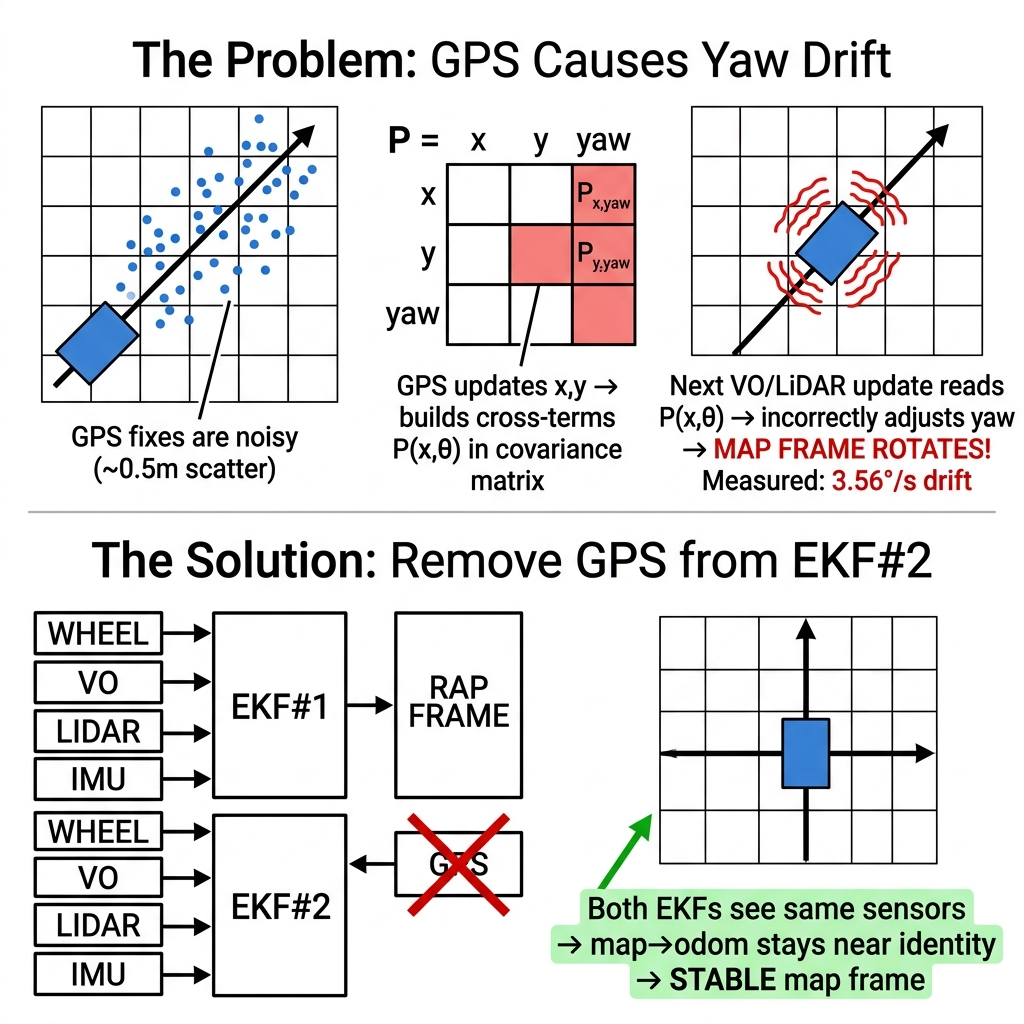
\includegraphics[width=0.85\textwidth]{figures/yaw_coupling_problem.png}
\caption{The GPS position--yaw covariance coupling problem. GPS corrections
build off-diagonal $\mathbf{P}_{x\theta}$ terms that leak into yaw when VO or
LiDAR updates are applied, causing sustained map-frame rotation at
$\sim$3.56$^\circ$/s.}
\label{fig:yawcoupling}
\end{figure}

\subsection{The Covariance Cross-Term Problem}

The EKF's state covariance matrix $\mathbf{P}$ has off-diagonal terms. When
GPS updates the position $(x, y)$, the Kalman gain computation involves
\emph{all} states, including yaw $\psi$. Over multiple GPS corrections, the
off-diagonal terms $P_{x,\psi}$ and $P_{y,\psi}$ grow. Then when a visual or
LiDAR odometry update arrives and corrects the position, the cross-terms cause
the EKF to \emph{also} adjust yaw---even though the VO/LiDAR update had
nothing to do with heading.

The result: the \texttt{map} frame slowly rotates. Measured drift:
$\approx 3.56^\circ$/s, which is catastrophic for any downstream navigation.

\subsection{The Solution: Sensor Consensus}

By giving EKF\,\#2 the \emph{same} sensor inputs as EKF\,\#1 (just in the
\texttt{map} world frame), both filters track nearly the same state. The
\texttt{map}$\rightarrow$\texttt{odom} transform stays near-identity:
$\pm 0.1$\,m translation, $\pm 1^\circ$ rotation over a 2-minute run.

The GPS data still flows through the system (navsat converts it to
\texttt{/odometry/gps}), but that topic is simply not listed in EKF\,\#2's
sensor inputs. It's available for analysis notebooks but doesn't corrupt the
map frame.

% ============================================================
\section{Step 7: The Complete Data Flow}
% ============================================================

\begin{figure}[H]
\centering
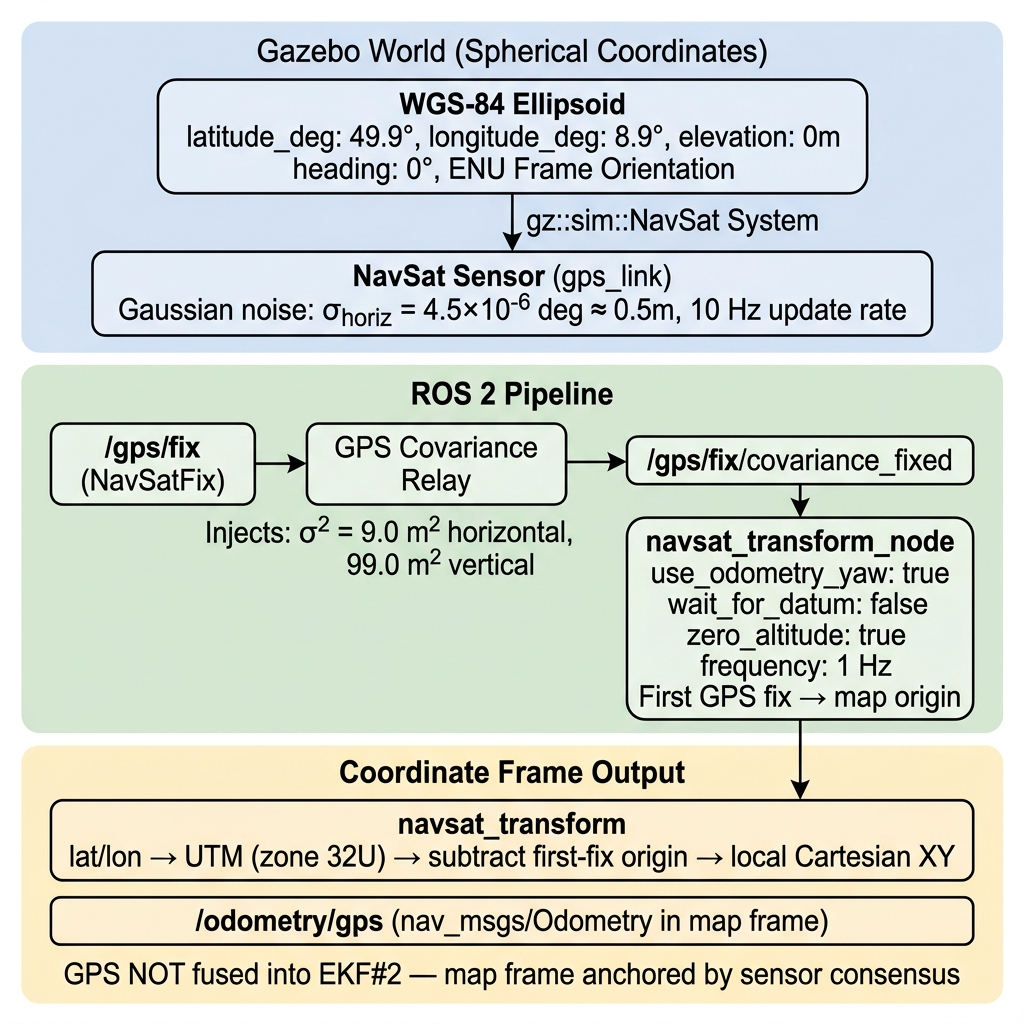
\includegraphics[width=0.85\textwidth]{figures/datum_projection_pipeline.png}
\caption{The complete GPS datum projection pipeline from Gazebo world
coordinates through the ROS\,2 processing chain.}
\label{fig:pipeline}
\end{figure}

Putting it all together, the data flows like this:

\begin{enumerate}[itemsep=4pt]
  \item \textbf{Gazebo physics} computes robot pose $(x, y, z)$ in meters.
  \item \textbf{NavSat plugin} converts to $(\varphi, \lambda)$ using WGS-84,
        adds noise ($\sigma = 0.5$\,m), publishes \texttt{/gps/fix}.
  \item \textbf{GPS Covariance Relay} injects realistic covariance
        ($\sigma^2 = 9.0$\,m$^2$), publishes \texttt{/gps/fix/covariance\_fixed}.
  \item \textbf{navsat\_transform} receives first fix $\rightarrow$ locks datum
        origin. Reads EKF\,\#1 heading ($\psi = 0$) $\rightarrow$ aligns axes.
        All future fixes: UTM project, subtract origin $\rightarrow$
        \texttt{/odometry/gps} in local meters.
  \item \textbf{EKF\,\#1} fuses wheel + VO + LiDAR + IMU in \texttt{odom}
        frame $\rightarrow$ publishes \texttt{odom}$\rightarrow$\texttt{base\_link}.
  \item \textbf{EKF\,\#2} fuses same sensors in \texttt{map} frame
        (NO GPS!) $\rightarrow$ publishes \texttt{map}$\rightarrow$\texttt{odom}.
\end{enumerate}

% ============================================================
\section{Step 8: The TF Frame Hierarchy}
% ============================================================

\begin{figure}[H]
\centering
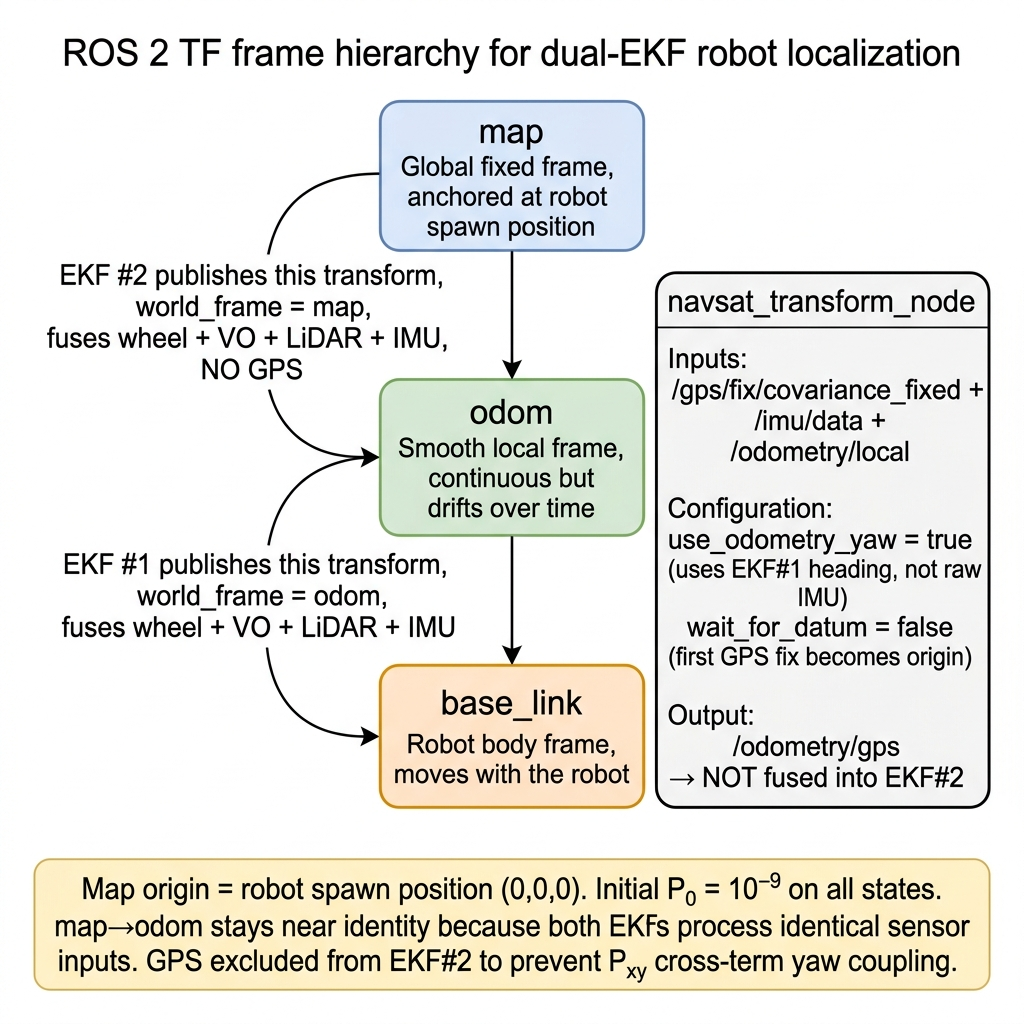
\includegraphics[width=0.85\textwidth]{figures/tf_frame_hierarchy.png}
\caption{The ROS\,2 TF frame hierarchy showing which node publishes each
transform, and how the navsat\_transform node feeds into (but is excluded
from) EKF\,\#2.}
\label{fig:tfhierarchy}
\end{figure}

\subsection{Initial Covariance: The $10^{-9}$ Lock}

Both EKFs set their initial state covariance to:
\begin{equation}
  \mathbf{P}_0 = 10^{-9} \cdot \mathbf{I}_{15}
\end{equation}

This is \emph{extremely} small---it tells the filter: ``I am almost perfectly
certain the robot is at $(0, 0, 0)$ with heading $0$.'' Why?

Because the robot \emph{is} at $(0, 0, 0)$---it just spawned there. With such
tight initial covariance:
\begin{itemize}
  \item The Kalman gain for any early measurement is $K \approx 10^{-10}$
  \item No single sensor can yank the state away from the known starting point
  \item Covariance grows gradually via process noise $\mathbf{Q}$, so sensors
        gain influence slowly and smoothly
\end{itemize}

% ============================================================
\section{RTAB-Map Visual Odometry (RGB-D)}
% ============================================================

The \texttt{rgbd\_odometry} node from the \texttt{rtabmap\_odom} package
estimates the robot's motion by tracking visual features across consecutive
camera frames. Fig.~\ref{fig:vo_pipeline} shows the complete pipeline.

\begin{figure}[H]
\centering
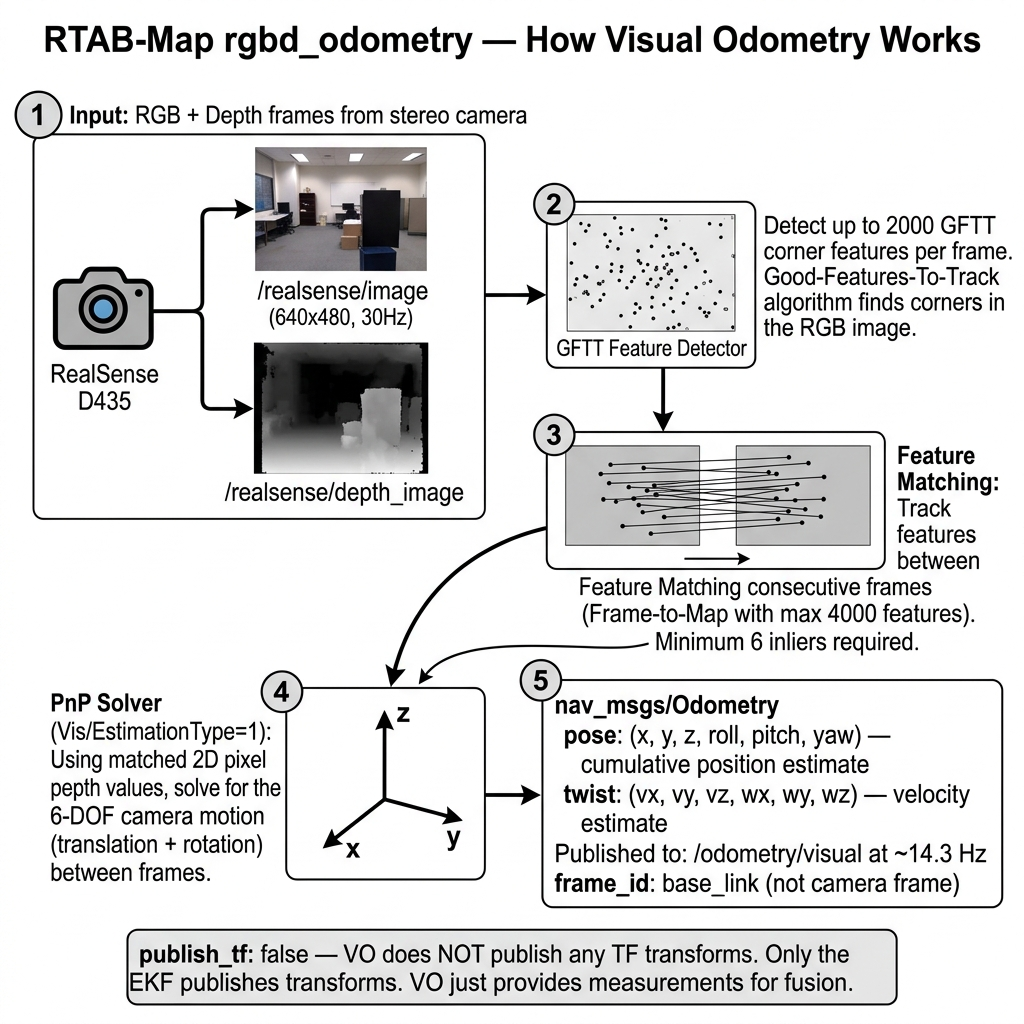
\includegraphics[width=0.85\textwidth]{figures/visual_odometry_pipeline.png}
\caption{RTAB-Map RGB-D visual odometry pipeline. The RealSense D435 provides
synchronized color and depth images. GFTT features are detected, matched across
frames, and a PnP solver recovers the 6-DOF camera motion.}
\label{fig:vo_pipeline}
\end{figure}

\subsection{Inputs}
\begin{itemize}[itemsep=2pt]
  \item \textbf{RGB image:} \texttt{/realsense/image} --- 640$\times$480
        color frame at 30\,Hz from the Intel RealSense D435.
  \item \textbf{Depth image:} \texttt{/realsense/depth\_image} --- aligned
        depth map, same resolution. Each pixel stores distance in meters
        (range: 0.105--10\,m).
  \item \textbf{Camera info:} \texttt{/realsense/camera\_info} --- intrinsic
        calibration ($f_x, f_y, c_x, c_y$, distortion). Needed to back-project
        2D pixels into 3D points.
\end{itemize}

\subsection{How It Works (Step by Step)}

\begin{enumerate}[itemsep=4pt]
  \item \textbf{Feature detection (GFTT):} The Good-Features-To-Track
        algorithm (Shi-Tomasi corners) finds up to 2000 corner points in the
        RGB image. Corners are places where intensity changes in two
        directions---intersections, edges of objects, texture boundaries.
        Your config uses \texttt{Vis/FeatureType: 0} = GFTT, and
        \texttt{Vis/MaxFeatures: 2000} (raised from default 1000 because
        the agriculture terrain is visually sparse).

  \item \textbf{Feature matching (Frame-to-Map):} Detected features are
        matched against a local map of previously seen features (up to 4000
        features in the map via \texttt{OdomF2M/MaxSize: 4000}). Matching
        uses descriptor similarity. At least 6 inlier matches are required
        (\texttt{Vis/MinInliers: 6})---if fewer are found, the frame is
        rejected and the odometry resets after 5 consecutive failures
        (\texttt{Odom/ResetCountdown: 5}).

  \item \textbf{3D point recovery:} For each matched 2D feature, the
        corresponding depth pixel provides the $Z$ distance. Combined with
        the camera intrinsics, this gives a 3D point $(X, Y, Z)$ in camera
        coordinates:
        \begin{equation}
          X = \frac{(u - c_x) \cdot Z}{f_x}, \quad
          Y = \frac{(v - c_y) \cdot Z}{f_y}
        \end{equation}

  \item \textbf{PnP solver:} With matched 2D$\leftrightarrow$3D
        correspondences, the Perspective-n-Point algorithm
        (\texttt{Vis/EstimationType: 1}) solves for the rigid-body transform
        $(R, t)$ that best explains the observed feature motion. This gives
        the 6-DOF camera displacement between frames.

  \item \textbf{Transform to base\_link:} The camera-frame displacement is
        transformed to \texttt{base\_link} using the known camera mount
        transform (the \texttt{body\_to\_camera\_joint} in the URDF: $x=0.38$,
        $z=0.20$, pitch $= 0.35$\,rad down).
\end{enumerate}

\subsection{Output}

A \texttt{nav\_msgs/Odometry} message on \texttt{/odometry/visual} at
$\sim$14.3\,Hz containing:
\begin{itemize}
  \item \textbf{pose:} Cumulative $(x, y, z, \text{roll}, \text{pitch}, \text{yaw})$
        --- the total displacement from where VO started.
  \item \textbf{twist:} Instantaneous $(v_x, v_y, v_z, \omega_x, \omega_y, \omega_z)$
        --- velocity computed from consecutive frame deltas.
  \item \textbf{covariance:} $6\times 6$ matrix auto-computed from the number
        of inliers and reprojection error.
  \item \textbf{frame\_id:} \texttt{base\_link} (not \texttt{camera\_link}).
\end{itemize}

\begin{warning}
\texttt{publish\_tf: false} --- The VO node does NOT publish any TF transforms.
Only the EKF publishes transforms. VO is purely a measurement source.
If this were \texttt{true}, you'd have two nodes fighting over the same
TF transform and the robot would jitter violently in RViz.
\end{warning}

% ============================================================
\section{RTAB-Map ICP LiDAR Odometry}
% ============================================================

The \texttt{icp\_odometry} node estimates motion by aligning consecutive 3D
LiDAR scans using the Iterative Closest Point algorithm.
Fig.~\ref{fig:icp_pipeline} shows the pipeline.

\begin{figure}[H]
\centering
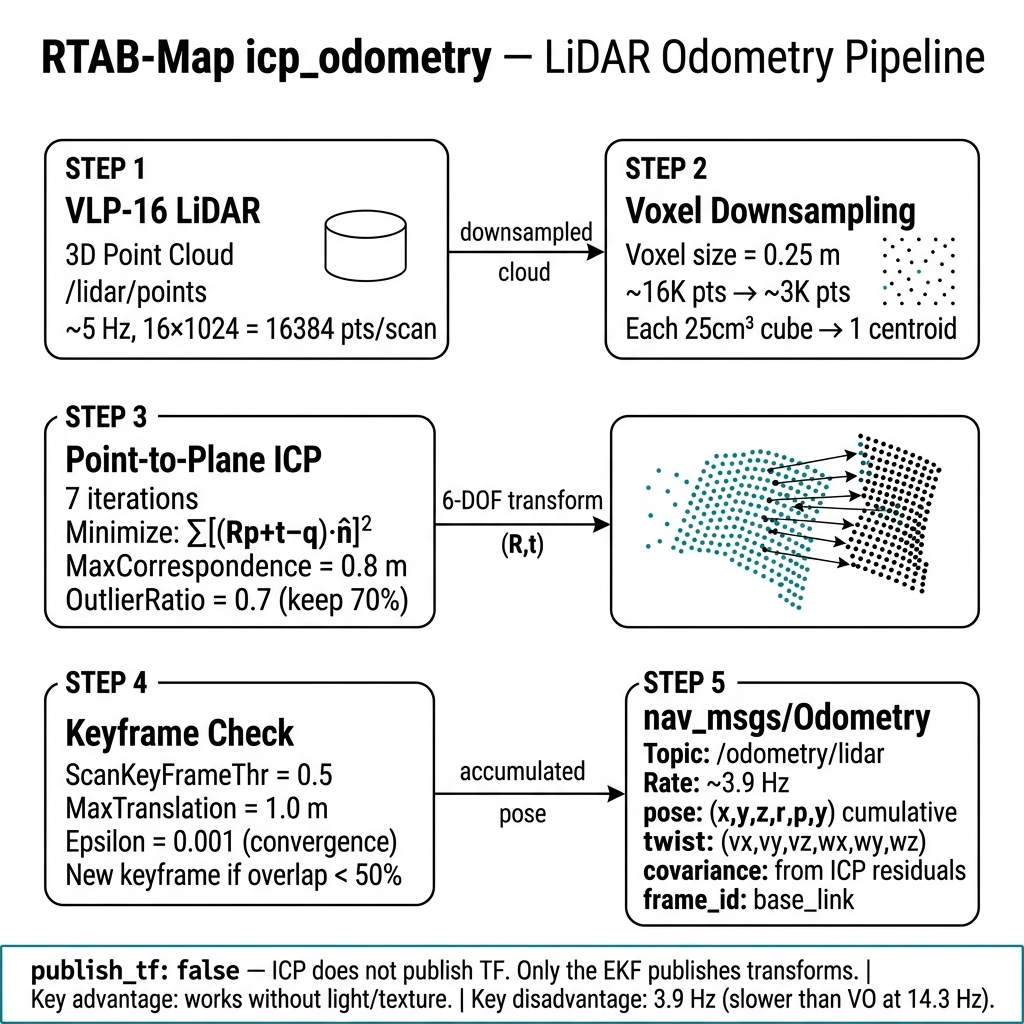
\includegraphics[width=0.85\textwidth]{figures/icp_odometry_pipeline.png}
\caption{RTAB-Map ICP LiDAR odometry pipeline. Point clouds from the VLP-16
are voxel-downsampled, then aligned to the previous scan using point-to-plane
ICP to recover 6-DOF motion.}
\label{fig:icp_pipeline}
\end{figure}

\subsection{Inputs}
\begin{itemize}
  \item \textbf{Point cloud:} \texttt{/lidar/points} ---
        \texttt{PointCloud2} from the VLP-16 at $\sim$5\,Hz.
        16 vertical beams $\times$ 1024 horizontal rays = up to 16384 points
        per scan, covering 360$^\circ$ horizontal, $\pm$15$^\circ$ vertical.
\end{itemize}

\subsection{How It Works (Step by Step)}

\begin{enumerate}[itemsep=4pt]
  \item \textbf{Voxel downsampling:} The raw cloud ($\sim$16K points) is
        divided into $0.25 \times 0.25 \times 0.25$\,m voxels
        (\texttt{Icp/VoxelSize: 0.25}). Each voxel keeps one representative
        point (centroid). Result: $\sim$2000--4000 points. This makes ICP
        faster and more robust to noise.

  \item \textbf{Point-to-Plane ICP:}
        (\texttt{Icp/PointToPlane: true}) --- For each point $\mathbf{p}_i$ in
        the current scan, find the closest point $\mathbf{q}_i$ in the previous
        scan. Compute the surface normal $\hat{\mathbf{n}}_i$ at $\mathbf{q}_i$.
        Then minimize:
        \begin{equation}
          \min_{R, t} \sum_i \left[ (R\,\mathbf{p}_i + t - \mathbf{q}_i) \cdot \hat{\mathbf{n}}_i \right]^2
        \end{equation}
        This is iterated 7 times (\texttt{Icp/Iterations: 7}). Point-to-plane
        converges faster than point-to-point because it allows points to
        ``slide'' along surfaces.

  \item \textbf{Outlier rejection:} Points whose correspondence distance
        exceeds 0.8\,m (\texttt{Icp/MaxCorrespondenceDistance}) are ignored.
        Additionally, 30\% of the worst-matching points are discarded
        (\texttt{Icp/OutlierRatio: 0.7} means keep 70\%).

  \item \textbf{Convergence check:} If the transform change between
        iterations drops below $\epsilon = 0.001$
        (\texttt{Icp/Epsilon}), ICP stops early. Max translation per
        step is clamped to 1.0\,m (\texttt{Icp/MaxTranslation}).

  \item \textbf{Keyframe management:} A new keyframe is created when the
        cumulative motion exceeds 50\% of the scan overlap
        (\texttt{Odom/ScanKeyFrameThr: 0.5}). Between keyframes, ICP
        aligns against the stored keyframe scan.
\end{enumerate}

\subsection{Output}

A \texttt{nav\_msgs/Odometry} message on \texttt{/odometry/lidar} at
$\sim$3.9\,Hz containing the same fields as visual odometry (pose, twist,
covariance), but with covariance auto-computed from the ICP residual error.

\subsection{Visual Odom vs.\ LiDAR Odom: Key Differences}

\begin{table}[H]
\centering
\begin{tabular}{@{}lcc@{}}
\toprule
\textbf{Property} & \textbf{Visual (RGB-D)} & \textbf{LiDAR (ICP)} \\
\midrule
Sensor & RealSense D435 & VLP-16 \\
Rate & $\sim$14.3\,Hz & $\sim$3.9\,Hz \\
Range & 0.1--10\,m & 0.4--100\,m \\
FOV & 87$^\circ$ $\times$ 57$^\circ$ & 360$^\circ$ $\times$ 30$^\circ$ \\
Failure mode & Featureless surfaces & Long featureless corridors \\
Yaw accuracy & Poor (agri terrain) & Good (360$^\circ$ scan) \\
EKF uses yaw? & \textbf{No} & \textbf{Yes} \\
\bottomrule
\end{tabular}
\caption{Comparison of the two RTAB-Map odometry sources.}
\end{table}

% ============================================================
\section{How the EKF Consumes Odometry: Differential Mode}
% ============================================================

Both VO and LiDAR odom are consumed with \texttt{differential: true}.
This is a crucial setting that determines \emph{how} the EKF interprets the
pose data (Fig.~\ref{fig:differential}).

\begin{figure}[H]
\centering
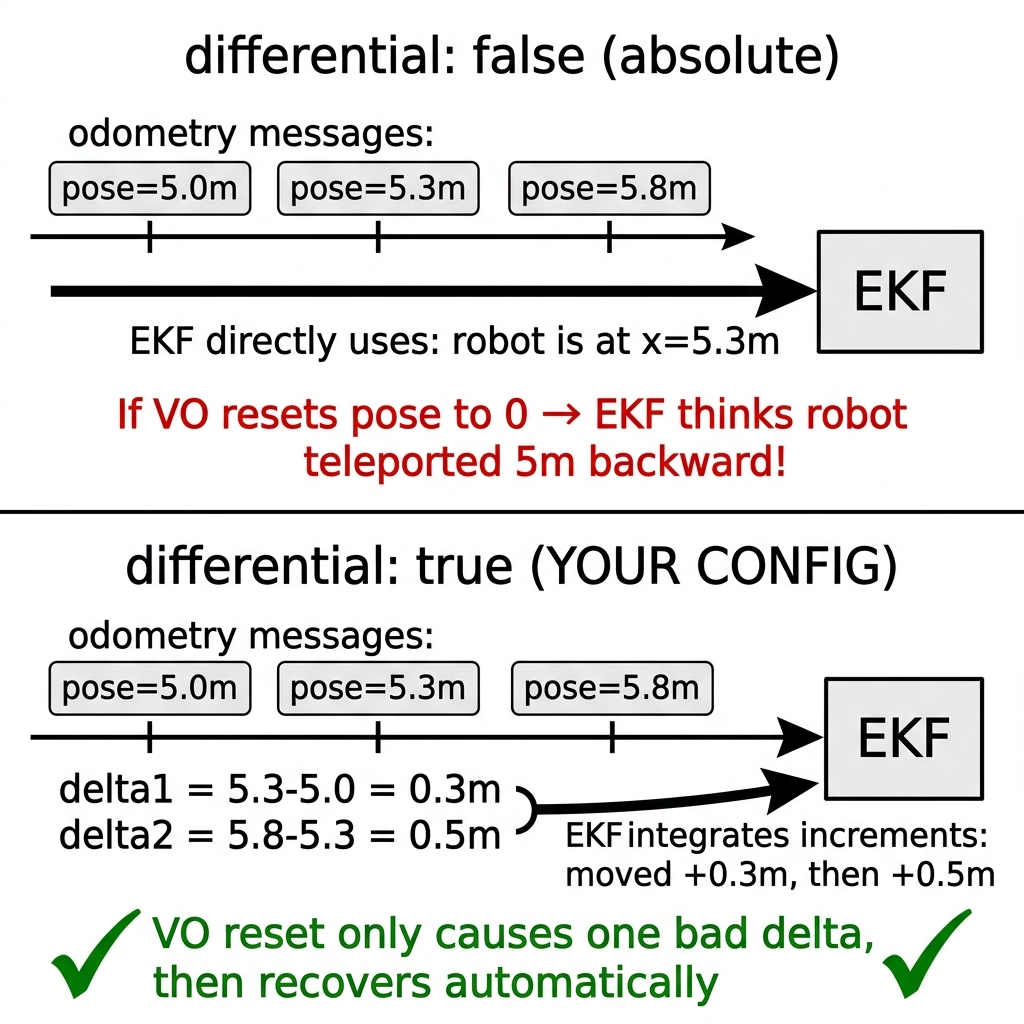
\includegraphics[width=0.8\textwidth]{figures/differential_mode.png}
\caption{Differential mode converts absolute poses to increments before EKF
fusion. This protects against VO/LiDAR resets corrupting the state estimate.}
\label{fig:differential}
\end{figure}

\begin{keyidea}
With \texttt{differential: true}, the EKF never sees ``robot is at position
$X$''---it only sees ``robot moved $\Delta X$ since the last message.'' This
means RTAB-Map can internally reset its pose estimate (after tracking
failures) without destroying the EKF state. Only one update will be wrong
(the delta spanning the reset), and the system self-recovers on the next
good frame.
\end{keyidea}

% ============================================================
\section{The Sensor Selection Matrix}
% ============================================================

The 15-element boolean \texttt{config} array for each sensor determines
exactly which fields the EKF reads. Fig.~\ref{fig:sensormatrix} shows the
full picture.

\begin{figure}[H]
\centering
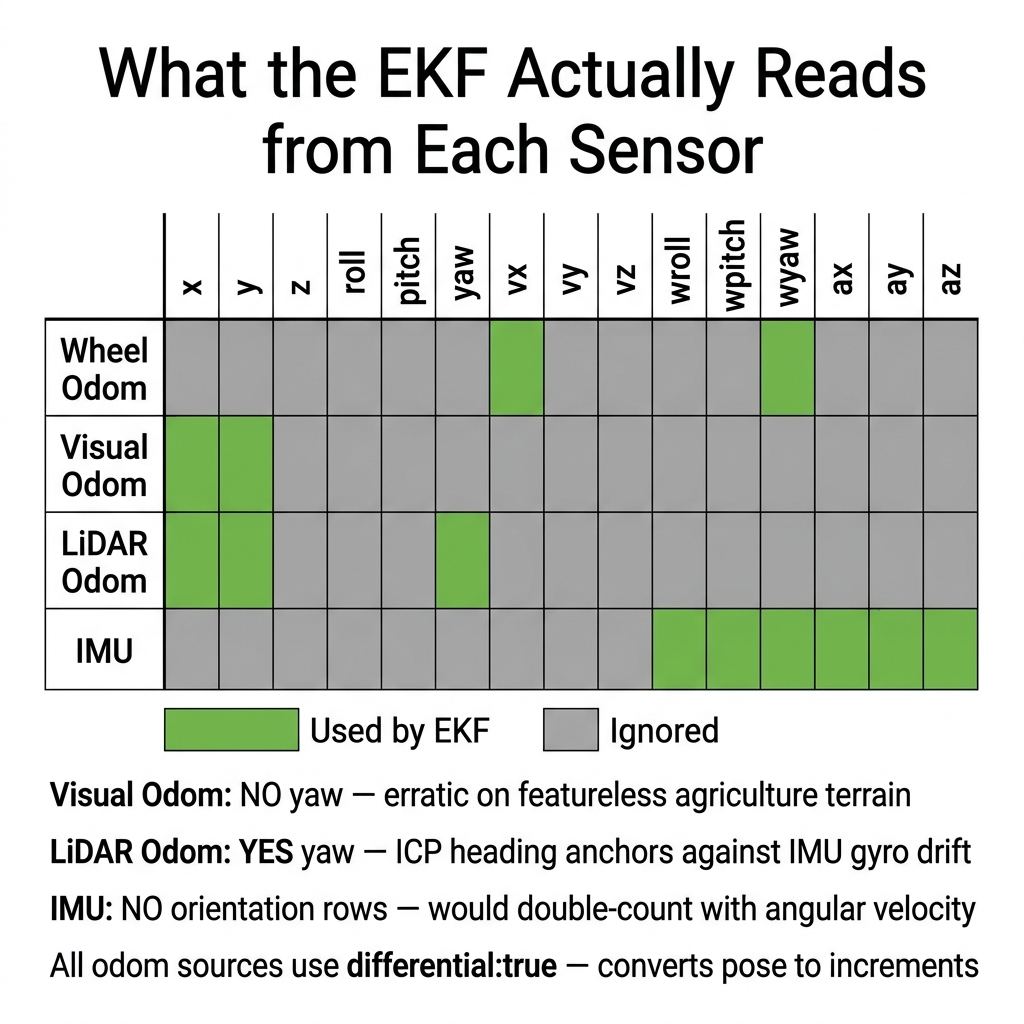
\includegraphics[width=0.85\textwidth]{figures/ekf_sensor_matrix.png}
\caption{Which state variables each sensor contributes to the EKF. Green =
used, grey = ignored. Note: VO provides no yaw (erratic on agriculture
terrain), while LiDAR provides yaw (reliable 360$^\circ$ ICP heading).}
\label{fig:sensormatrix}
\end{figure}

Key design decisions in the sensor matrix:
\begin{itemize}[itemsep=4pt]
  \item \textbf{Wheel odom:} Only $v_x$ and $\omega_z$ (velocities). Position
        is not used because wheel odometry position accumulates unbounded
        drift from wheel slip.
  \item \textbf{Visual odom:} Only $x, y$ (position, differential).
        \textbf{No yaw} --- on the featureless agriculture terrain, VO heading
        estimates oscillate by 50$^\circ$+ and corrupt the EKF.
  \item \textbf{LiDAR odom:} $x, y$ \textbf{and yaw} (differential).
        ICP on 360$^\circ$ scans gives reliable heading that anchors against
        IMU gyro bias drift ($\sim$3$^\circ$/min without it).
  \item \textbf{IMU:} Angular velocity ($\omega_x, \omega_y, \omega_z$) and
        linear acceleration ($a_x, a_y, a_z$). \textbf{No orientation rows}
        --- fusing both orientation and angular velocity would double-count the
        same gyroscope signal, amplifying bias.
\end{itemize}

% ============================================================
\section{Summary: Your Config Decisions at a Glance}
% ============================================================

\begin{table}[H]
\centering
\small
\begin{tabular}{@{}p{5cm}p{3cm}p{6cm}@{}}
\toprule
\textbf{Parameter} & \textbf{Your Value} & \textbf{Effect} \\
\midrule
\texttt{spherical\_coordinates} & 49.9°N, 8.9°E & Gazebo world origin on WGS-84 \\
\texttt{world\_frame\_orientation} & ENU & $+X$=East, $+Y$=North, $+Z$=Up \\
NavSat noise $\sigma$ & $4.5\times10^{-6}$\,deg & $\approx 0.5$\,m GPS scatter \\
\texttt{wait\_for\_datum} & \texttt{false} & First GPS fix = map origin \\
\texttt{use\_odometry\_yaw} & \texttt{true} & Heading from EKF\,\#1 (not IMU) \\
\texttt{zero\_altitude} & \texttt{true} & Forces $z = 0$ in GPS output \\
\texttt{two\_d\_mode} & \texttt{true} & 15D $\rightarrow$ 6D state \\
EKF\,\#1 \texttt{world\_frame} & \texttt{odom} & Publishes odom$\rightarrow$base\_link \\
EKF\,\#2 \texttt{world\_frame} & \texttt{map} & Publishes map$\rightarrow$odom \\
GPS in EKF\,\#2 & \textbf{excluded} & Prevents $P_{x\theta}$ yaw coupling \\
$\mathbf{P}_0$ diagonal & $10^{-9}$ & Locks to known spawn position \\
NavSat frequency & 1\,Hz & Slow GPS $\rightarrow$ less map jitter \\
\bottomrule
\end{tabular}
\caption{All datum and frame-related configuration decisions.}
\end{table}

\end{document}
